\subsubsection{Combining batch and stream: Lambda Architecture}

\definition{Lambda architecture} is a \textbf{data-processing architecture} designed to handle massive quantities of data by taking advantage of both batch and stream-processing methods. 

\highspace
This approach to architecture attempts to balance latency, throughput, and fault-tolerance by using batch processing to provide comprehensive and accurate views of batch data, while simultaneously using real-time stream processing to provide views of online data. The two view outputs may be joined before presentation. 

\highspace
The rise of lambda architecture is correlated with the growth of big data, real-time analytics, and the drive to mitigate the latencies of map-reduce.

\begin{figure}[!htp]
    \centering
    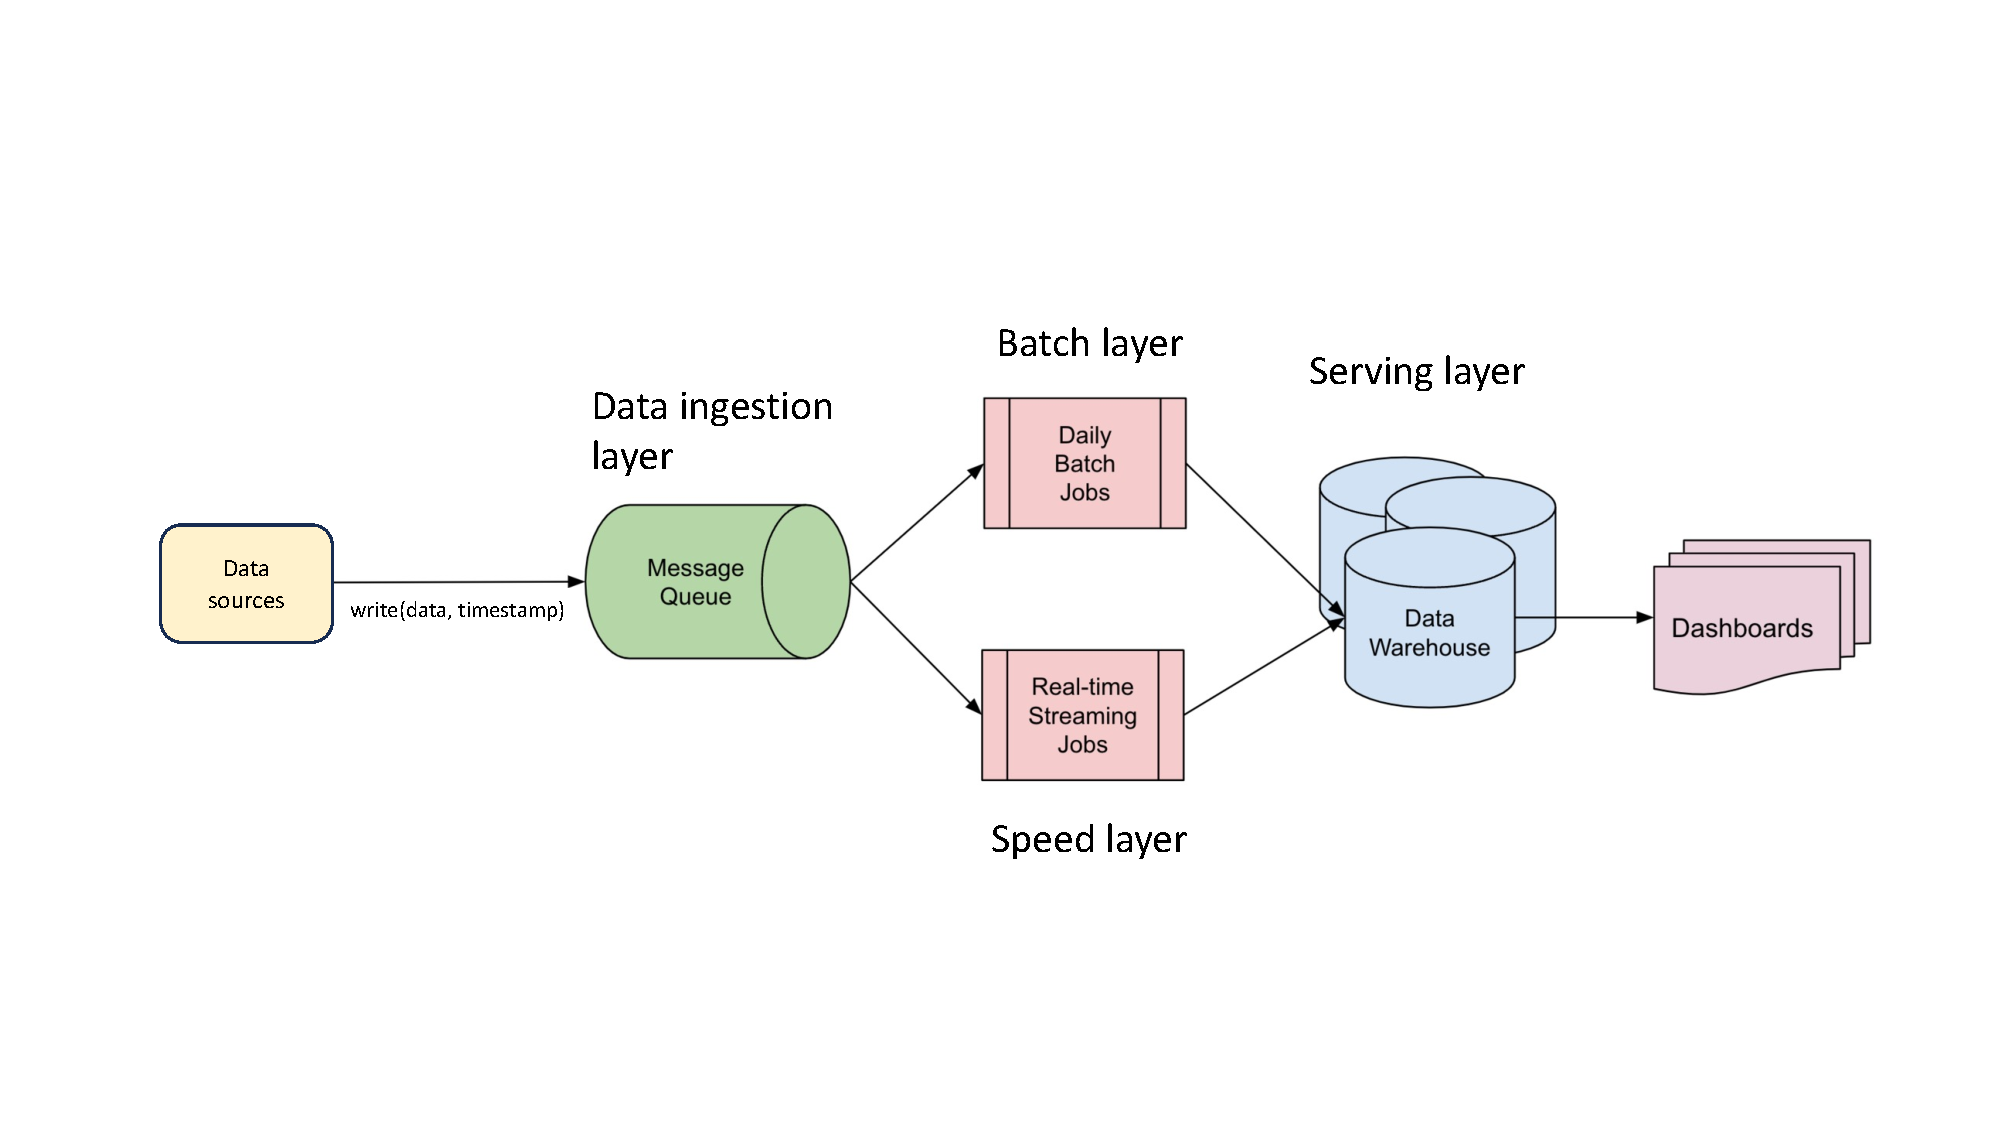
\includegraphics[width=\textwidth]{img/lambda-arch.pdf}
    \caption{Lambda architecture.}
\end{figure}

Exist also \definition{Kappa architecture}. Kappa architecture is a software architecture used for processing streaming data with a single technology stack. It is a simplification of Lambda architecture, where the data is processed in batches. Kappa architecture ingests data into a messaging system like Apache Kafka, and performs both real-time and batch processing, especially for analytics, on the same stream. It allows for recomputation on the data by streaming it through the pipeline again.